%% This Beamer template is based on the one found here: https://github.com/sanhacheong/stanford-beamer-presentation, and edited to be used for Stanford ARM Lab

\documentclass[10pt]{beamer}
%\mode<presentation>{}

\usepackage{media9}
\usepackage{amssymb,amsmath,amsthm,enumerate}
\usepackage{mathtools}
\usepackage[utf8]{inputenc}
\usepackage{array}
\usepackage[parfill]{parskip}
\usepackage[utf8]{vietnam}
\usepackage{graphicx,animate}
\usepackage{caption}
\usepackage{subcaption}
\usepackage{bm}
\usepackage{amsfonts,amscd}
\usepackage[]{units}
\usepackage{listings}
\usepackage{multicol}
\usepackage{multirow}
\usepackage{tcolorbox}
\usepackage{physics}
\usepackage{movie15}
% Enable colored hyperlinks
\hypersetup{colorlinks=true}

\usefonttheme{professionalfonts}

% The following three lines are for crossmarks & checkmarks
\usepackage{pifont}% http://ctan.org/pkg/pifont
\newcommand{\cmark}{\ding{51}}%
\newcommand{\xmark}{\ding{55}}%

% Numbered captions of tables, pictures, etc.
\setbeamertemplate{caption}[numbered]
\usepackage{media9} 
%\usepackage[superscript,biblabel]{cite}
%\usepackage{algorithmic}
%\usepackage{algorithm2e}
%\usepackage{algpseudocode}
\usepackage[linesnumbered,ruled,vlined]{algorithm2e}
%\usepackage{algorithm}
%\usepackage{algorithmic}
%\usepackage{caption}
\usepackage[font=scriptsize,justification=centering]{caption}
%\usepackage{xcolor}
\usepackage{array}
%\renewcommand{\thealgocf}{}

\usepackage[natbib,backend=biber,style=ieee, sorting=ynt]{biblatex}
\bibliography{ref.bib}

\usepackage[acronym]{glossaries}

\usepackage{graphicx}
\graphicspath{{./figures}}
\usepackage{hyperref}

\usepackage{pythonhighlight}

\setbeamertemplate{theorems}[numbered]
\theoremstyle{remark}
\newtheorem{dl}{Định lý}
\newtheorem{md}{Mệnh đề}
\newtheorem{bd}{Bổ đề}
\newtheorem{dn}{Định nghĩa}
\newtheorem{hq}{Hệ quả}
%\theoremstyle{definition}

\numberwithin{algocf}{section}
\numberwithin{equation}{section}
\numberwithin{dl}{section}
\numberwithin{figure}{section}


%\newcommand{\empy}[1]{{\color{darkorange}\emph{#1}}}
%\newcommand{\empr}[1]{{\color{cardinalred}\emph{#1}}}
%\newcommand{\examplebox}[2]{
%\begin{tcolorbox}[colframe=darkcardinal,colback=boxgray,title=#1]
%#2
%\end{tcolorbox}}

%\usetheme{Stanford} 
%\input{./style_files_stanford/my_beamer_defs.sty}
\usetheme{Copenhagen}
\usecolortheme{seahorse}
%\logo{
\includegraphics[height=0.5in]{logos/HUS-name.jpg}}

\makeatletter
\let\@@magyar@captionfix\relax
\makeatother

\title[Mô hình sinh dựa trên điểm số]{Mô hình sinh dựa trên điểm số bằng phương trình vi phân ngẫu nhiên}

\AtBeginSection[]
{
    \begin{frame}[shrink]
        \frametitle{Nội dung}
        \tableofcontents[currentsection, subsectionstyle=show/show/hide]
    \end{frame}
}

\setbeamertemplate{page number in head/foot}[totalframenumber]
\setbeamertemplate{frametitle continuation}{}

\begin{document}
\author[Nguyễn Chí Thanh - 21007925]{
	\begin{tabular}{c} 
	\Large
	Nguyễn Chí Thanh \\
    \footnotesize \href{mailto:nguyenchithanh\_sdh21@hus.edu.vn}{nguyenchithanh\_sdh21@hus.edu.vn}
\end{tabular}
\vspace{-4ex}}

\institute{
	\vskip 5pt
	\begin{figure}
		\centering
		\begin{subfigure}[t]{0.5\textwidth}
			\centering
			
\includegraphics[height=0.75in]{logos/HUS-logo.jpg}
		\end{subfigure}%
		~ 
		\begin{subfigure}[t]{0.5\textwidth}
			\centering
			
\includegraphics[height=0.75in]{logos/MIM-logo.png}
		\end{subfigure}
	\end{figure}
	\vskip 5pt	
	Đại học Quốc Gia Hà Nội \\
	Trường đại học Khoa học tự nhiên\\
	Khoa Toán - Cơ - Tin học
	\vskip 3pt
}

%\begin{noheadline}
\begin{frame}[shrink] \maketitle \end{frame}
%\end{noheadline}
    
\setbeamertemplate{itemize items}[default]
\setbeamertemplate{itemize subitem}[circle]

\begin{frame}{Nội dung}
    \tableofcontents[hidesubsections]
\end{frame}

\section{Tổng quan mô hình sinh dựa trên điểm số}

\begin{frame}{Tổng quan mô hình khuếch tán}
	Quá trình khuếch tán gồm hai quá trình:
	\begin{itemize}
		\item Quá trình khuếch tán thuận: nhiễu được từ từ thêm vào dữ liệu qua từng bước cho đến khi dữ liệu trở thành nhiễu có phân phối biết trước (thường là phân phối chuẩn tắc)
		\item Quá trình khuếch tán ngược (quá trình khử nhiễu): sử dụng một mô hình được huấn luyện đảo ngược quá trình thuận (từ nhiễu trở thành dữ liệu)
	\end{itemize}
	\begin{figure}[H]
		\centering
		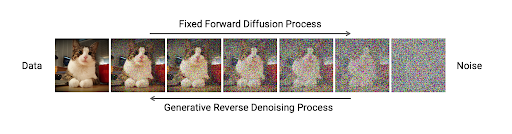
\includegraphics[width=0.9\linewidth]{figures/Fixed_Forward_Diffusion_Process.png}
	\end{figure}
\end{frame}

\begin{frame}{Tổng quan mô hình sinh dựa trên điểm số}
	\begin{itemize}
		\item Mô hình sinh dựa trên điểm số là các mô hình tạo ra dữ liệu cần thông tin về gradient của $\log$ hàm mật độ xác suất $p_t(\bold{x}_t)$
		\item Các mô hình sinh dựa trên điểm số hướng nghiên cứu chính về cách định nghĩa một quá trình làm xáo trộn dữ liệu (quá trình khuếch tán thuận) và cách tạo ra mẫu dữ liệu từ quá trình ngược tương ứng
		\item Các kỹ thuật (hàm mục tiêu) để ước lượng điểm số.
		\item Quá trình lấy mẫu có dạng một vòng lặp làm tăng độ hợp lý của mẫu dữ liệu. Ví dụ:
		\begin{equation*}
			\bold{x}_i = \bold{x}_{i-1} + \epsilon_i \nabla_{\bold{x}_{i-1}} p_{i-1}(\bold{x}_{i-1}) + \sqrt{2 \epsilon_i} \bold{z}_i, m = 1, 2, \dots, M
		\end{equation*}
	\end{itemize}
\end{frame}

\subsection{Score Matching with Langevin Dynamics (SMLD)}

\begin{frame}{Score Matching with Langevin Dynamics (SMLD)}
    \begin{itemize}
		\item Quá trình khuếch tán thuận:
		\begin{equation*}
			p_{\sigma}(\tilde{\bold{x}} \vert \bold{x}) \vcentcolon = \mathcal{N}(\tilde{\bold{x}};\bold{x}, \sigma^2 \bold{I})
		\end{equation*}
		\item Một dãy các ngưỡng nhiễu $\sigma_{\min} = \sigma_1 < \sigma_2 < \dots < \sigma_N = \sigma_{\max}$.
		\item $\sigma_{\min}$ đủ nhỏ để $p_{\sigma_{\min}} \approx p_{\mathrm{data}}(\bold{x})$, và $\sigma_{\max}$ đủ lớn để $p_{\sigma_{\max}}\approx \mathcal{N}(\bold{x}; \bold{0}, \sigma_{\max}^2 \bold{I})$
		\item \citep{song2019generative} sử dụng một mạng điểm số điều kiện trên nhiễu (Noise Conditional Score Network - NCSN), ký hiệu $\bold{s}_{\boldsymbol{\theta}}(\bold{x}, \sigma)$, được huấn luyện bởi hàm mục tiêu:
		\begin{equation} \label{eq:1}
			\boldsymbol{\theta}^{\ast} = \underset{\boldsymbol{\theta}}{\mathrm{argmin}} \sum_{i=1}^N \sigma_i^2 \mathbb{E}_{p_{\mathrm{data}}(\bold{x})} \mathbb{E}_{p_{\sigma_i}(\tilde{\bold{x}} \vert \bold{x})} \big\lbrack \lVert \bold{s}_{\boldsymbol{\theta} (\tilde{\bold{x}}, \sigma_i)} - \nabla_{\tilde{\bold{x}}} \log p_{\sigma_i} (\tilde{\bold{x}} \vert \bold{x})  \rVert_2^2 \big\rbrack
		\end{equation}
	\end{itemize}
\end{frame}

\begin{frame}{Score Matching with Langevin Dynamics (SMLD)}
	\begin{itemize}
		\item Quá trình khuếch tán ngược, khi ta đã huấn luyện mô hình điểm số $\bold{s}_{\boldsymbol{\theta}^{\ast}}(\bold{x}, \sigma)$ khớp với $\nabla_{\bold{x}} \log p_{\sigma}(\bold{x})$ tại hầu hết vị trí với $\sigma \in \lbrace \sigma_i \rbrace_{i=1}^N$.
		\item Để lấy mẫu, \citep{song2019generative} chạy M bước của Langevin MCMC để thu được mẫu dữ liệu cho lần lượt từng $p_{\sigma_i}(\bold{x})$:
		\begin{equation} \label{eq:2}
			\bold{x}_i^m = \bold{x}_i^{m-1} + \epsilon_i \bold{s}_{\boldsymbol{\theta}^{\ast}} (\bold{x}_i^{m-1}, \sigma_i) + \sqrt{2 \epsilon_i} \bold{z}_i^m, m = 1, 2, \dots, M
		\end{equation}
		với $\epsilon_i > 0$ là độ dài bước và $\bold{z}_i^m$ là một biến tuân theo phân phối chuẩn tắc.
		\ref{eq:2} được lặp lại cho $i=N, N-1, \dots, 1$ với $\bold{x}_N^0 \sim \mathcal{N}(\bold{x} \vert \bold{0}, \sigma_{\max}^2 \bold{I})$ và $\bold{x}_i^0 = \bold{x}_{i+1}^M$ khi $i < N$.
	\end{itemize}
\end{frame}

\subsection{Denoising Diffusion Probabilistic Model (DDPM)}

\begin{frame}{Denoising Diffusion Probabilistic Model (DDPM)}
	\begin{itemize}
		\item \citep{sohl2015deep,ho2020denoising} xét một dãy các ngưỡng nhiễu dương $0 < \beta_1, \beta_2, \dots, \beta_N < 1$.
		\item $\bold{x}_0 \sim p_{\mathrm{data}}(\bold{x})$, một xích Markov rời rạc $\lbrace \bold{x}_1, \bold{x}_2, \dots, \bold{x}_N \rbrace$ được tạo ra sao cho $p(\bold{x}_i \vert \bold{x}_{i-1}) = \mathcal{N}(\bold{x}_i; \sqrt{1-\beta_i} \bold{x}_{i-1}, \beta_i \bold{I})$
		\item $p_{\alpha_i}=\mathcal{N}(\bold{x}_i; \sqrt{\alpha_i}\bold{x}_0, (1-\alpha_i)\bold{I})$,
		với $\alpha_i \vcentcolon = \prod_{j=1}^i (1 - \beta_j)$
		\item Các mức nhiễu được chọn sao cho $\bold{x}_N$ có phân phối xấp xỉ phân phối chuẩn tắc $\mathcal{N}(\bold{0}, \bold{I})$.
		\item Quá trình khuếch tán ngược được tham số hóa với: $p_{\boldsymbol{\theta}} (\bold{x}_{i-1} \vert \bold{x}_i)=\mathcal{N}\Big(\bold{x}_{i-1}; \dfrac{1}{\sqrt{1-\beta_i}}(\bold{x}_i + \beta_i \bold{s}_{\boldsymbol{\theta}}(\bold{x}_i, i)), \beta_i \bold{I}\Big)$
		
	\end{itemize}
\end{frame}

\begin{frame}{Denoising Diffusion Probabilistic Model (DDPM)}
	\begin{itemize}
		\item Mạng ước lượng điểm số được huấn luyện với hàm mục tiêu:
		\begin{equation} \label{eq:3}
			\boldsymbol{\theta}^{\ast} = \underset{\boldsymbol{\theta}}{\mathrm{argmin}} \sum_{i=1}^N (1 - \alpha_i) \mathbb{E}_{p_{\mathrm{data}}(\bold{x})} \mathbb{E}_{p_{\alpha_i (\tilde{\bold{x}} \vert \bold{x})}} \big \lbrack \lVert \bold{s}_{\boldsymbol{\theta}} (\tilde{\bold{x}}, i) - \nabla_{\tilde{\bold{x}}} \log p_{\alpha_i} (\tilde{\bold{x}} \vert \bold{x}) \rVert_2^2 \big \rbrack
		\end{equation}
		\item Sau khi thu được mô hình tối ưu $\bold{s}_{\boldsymbol{\theta}^{\ast}}(\bold{x}, i)$, sử dụng công thức ước lượng xích Markov ngược:
		\begin{equation} \label{eq:4}
			\bold{x}_{i-1} = \dfrac{1}{\sqrt{1-\beta_i}} \big( \bold{x}_i + \beta_i \bold{s}_{\boldsymbol{\theta}^{\ast}} (\bold{x}_i, i) \big) + \sqrt{\beta_i} \bold{z}_i, i = N, N-1, \dots, 1
		\end{equation}
		với $\bold{x}_N \sim \mathcal{N}(\bold{0}, \bold{I}), \bold{z}_i \sim \mathcal{N}(\bold{0}, \bold{I})$. Phương pháp này được gọi là \textit{ancestral sampling}
	\end{itemize}
\end{frame}

\subsection{Mô hình sinh dựa trên phương trình vi phân tổng quát (SDE)}

\begin{frame}{Mô hình sinh dựa trên phương trình vi phân tổng quát (SDE)}
	\begin{figure}[H]
		\centering
		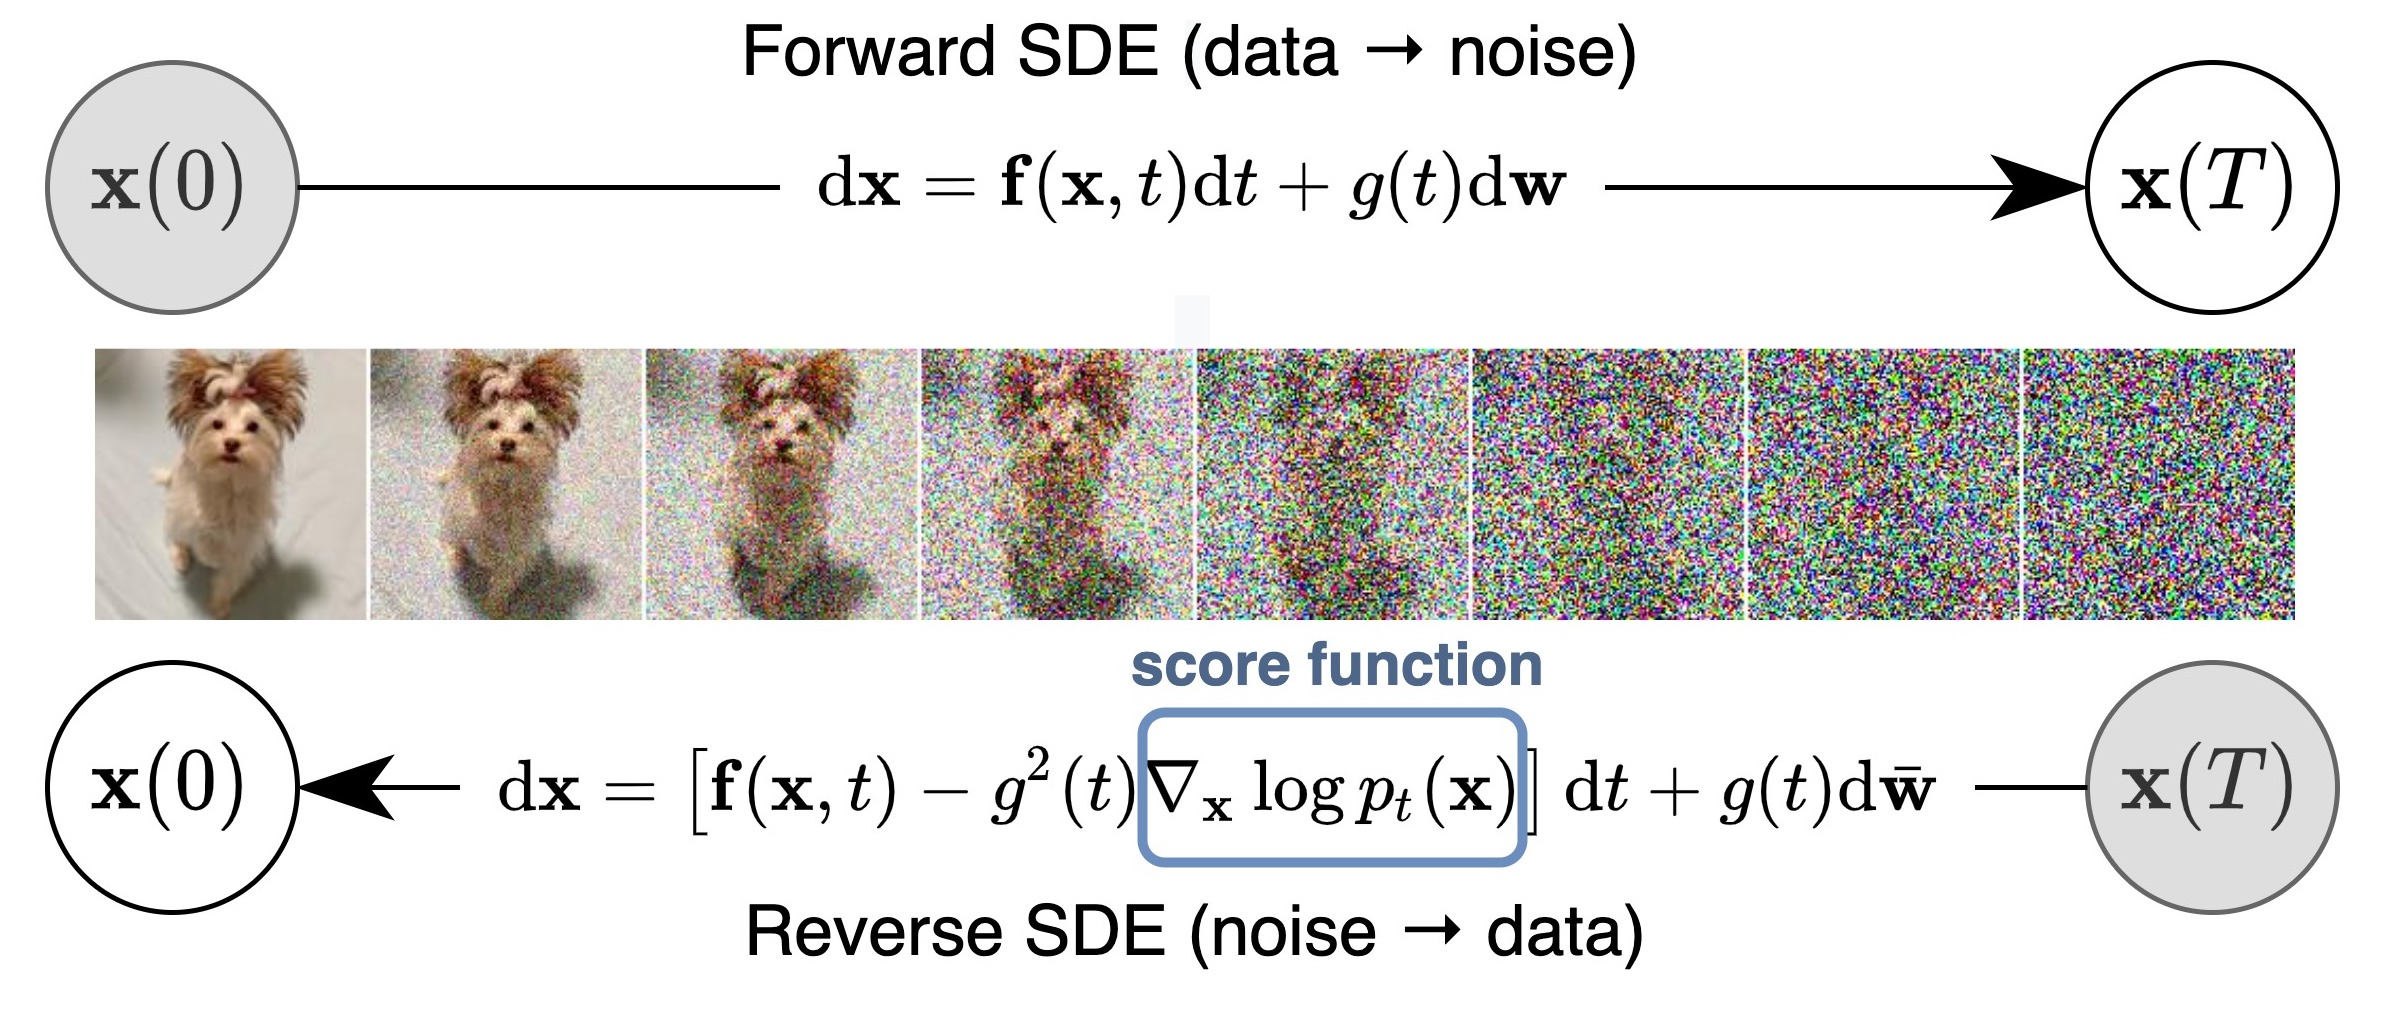
\includegraphics[width=0.8\textwidth]{1.jpg}
		\caption{Giải một phương trình SDE đảo ngược thời gian thu được một mô hình sinh dựa trên điểm.}
		\label{fig:1}
	\end{figure}
\end{frame}

\begin{frame}{Mô hình sinh dựa trên phương trình vi phân tổng quát (SDE)}
	\begin{figure}[H]
		\centering
		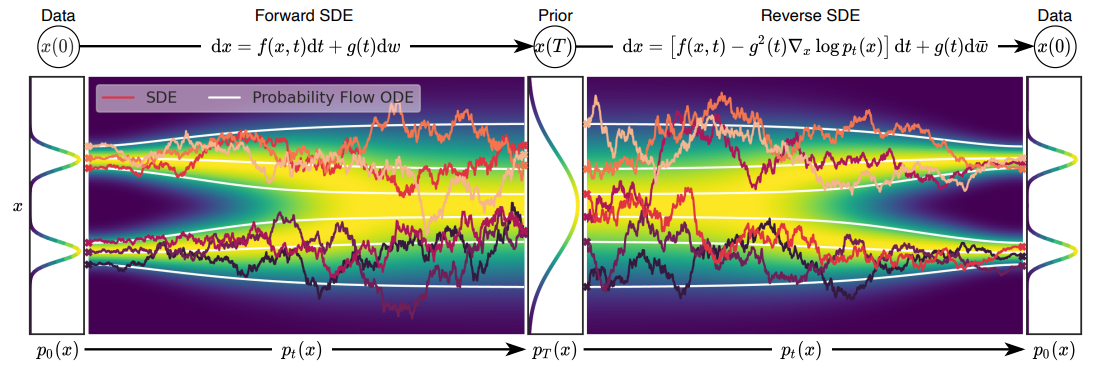
\includegraphics[width=\textwidth]{2.png}
		\caption{Tổng quan của một mô hình sinh dựa trên điểm số với phương trình SDE}
		\label{fig:2}
	\end{figure}
\end{frame}

\begin{frame}{Làm xáo trộn dữ liệu với phương trình SDE}
	\begin{itemize}
		\item $\lbrace \bold{x}(t) \rbrace_{t=0}^T$ được đánh chỉ số bởi một biến thời gian liên tục $t \in \lbrack 0, T \rbrack$
		\item $\bold{x}(0) \sim p_0$ là phân phối dữ liệu
		\item $\bold{x}(T) \sim p_T$ là phân phối tiên nghiệm được chọn trước thường là $\mathcal{N}(\bold{0}, \bold{I})$
		\item Quá trình khuếch tán có thể được mô hình hóa là nghiệm của phương trình Ito SDE:
		\begin{equation} \label{eq:5}
			d \bold{x} = \bold{f} (\bold{x}, t) dt + g(t) d \bold{w}
		\end{equation}
		với $\bold{w}$ là một quá trình Wiener chuẩn tắc (hay còn được gọi là chuyển động Brown), $\bold{f}(.,t): \mathbb{R}^d \rightarrow \mathbb{R}^d$ là một hàm vector được gọi là hệ số độ trôi của $\bold{x}(t)$ và $g(.): \mathbb{R} \rightarrow \mathbb{R}$ là một hàm vô hướng được gọi là hệ số khuếch tán của $\bold{x}(t)$.
	\end{itemize}
\end{frame}

\begin{frame}{Sinh mẫu dữ liệu bằng cách đảo ngược phương trình SDE}
	\begin{itemize}
		\item Từ các mẫu dữ liệu nhiễu $\bold{x}(T) \sim p_T$ và đảo ngược quá trình, ta có thể thu được các mẫu $\bold{x}(0) \sim p_0$.
		\item Đảo ngược một quá trình khuếch tán cũng là một quá trình khuếch tán, đi ngược theo thời gian bởi một phương trình SDE đảo ngược thời gian \citep{anderson1982reverse}:
		\begin{equation} \label{eq:6}
			d \bold{x} = \big \lbrack \bold{f}(\bold{x}, t) - g(t)^2 \nabla_{\bold{x}} \log p_t (\bold{x}) \big \rbrack dt + g(t) d \hat{\bold{w}}
		\end{equation}
		với $\hat{\bold{w}}$ là một quá trình Wiener chuẩn tắc khi thời gian đi ngược từ $T$ về $0$, và $dt$ là một vi phân gia số thời gian âm.
	\end{itemize}
\end{frame}

\begin{frame}[shrink]{Ước lượng điểm số cho phương trình SDE}
	\begin{itemize}
		\item Để ước lượng $\nabla_{\bold{x}} \log p_t(\bold{x})$, ta có thể huấn luyện một mô hình dựa trên điểm số phụ thuộc vào thời gian $\bold{s}_{\boldsymbol{\theta}}(\bold{x}, t)$ thông qua một tổng quát hóa liên tục từ công thức \ref{eq:1} và công thức \ref{eq:3}:
		\begin{equation} \label{eq:7}
			\boldsymbol{\theta}^{\ast} = \underset{\boldsymbol{\theta}}{\mathrm{argmin}} \mathbb{E}_t \Big \lbrace  \lambda(t) \mathbb{E}_{\bold{x}(0)} \mathbb{E}_{\bold{x}(t) \vert \bold{x}(0)} \big \lbrack \lVert \bold{s}_{\boldsymbol{\theta}} (\bold{x}(t), t) - \nabla_{\bold{x}(t)} \log p_{0t} (\bold{x}(t) \vert \bold{x}(0)) \rVert_2^2 \big \rbrack \Big \rbrace
		\end{equation}
		với $\lambda: \lbrace 0, T \rbrace \rightarrow \mathbb{R}_{>0}$ là một hàm trọng số dương,
		$t$ được lấy mẫu theo phân phối đều trên đoạn $\lbrace 0, T \rbrace$, $\bold{x}(0) \sim p_0 (\bold{x})$ và $\bold{x}(t) \sim p_{0t} (\bold{x}(t) \vert \bold{x}(0))$.
		\item Trong SMLD và DDPM, ta thường chọn $\lambda \propto 1 / \mathbb{E} \big \lbrack \lVert \nabla_{\bold{x}(t)} \log p_{0t} (\bold{x}(t) \vert \bold{x}(0)) \rVert_2^2 \big \rbrack$.
		\item Nếu $\bold{f}(.,t)$ là hàm affine, nhân chuyển tiếp luôn luôn là phân phối Gaussian.
		\item Với phương trình SDE tổng quát hơn, ta có thể giải phương trình Kolmogorov thuận \citep{oksendal2003stochastic} để thu được $p_{0t} (\bold{x}(t) \vert \bold{x}(0))$.
	\end{itemize}
\end{frame}

\subsection{Liên hệ với SMLD, DDPM}

\begin{frame}{Liên hệ với SMLD}
	\begin{itemize}
		\item Khi ta sử dụng $N$ mức nhiễu, từng nhân xáo trộn dữ liệu $p_{\sigma_i}(\bold{x} \vert \bold{x}_0)$ của SMLD tương ứng với phân phối của $\bold{x}_i$ theo xích Markov sau:

		\begin{equation}
		    \bold{x}_i = \bold{x}_{i-1} + \sqrt{\sigma_i^2 - \sigma_{i-1}^2} \bold{z}_{i-1}, i=1, \dots, N
		\end{equation}
		\item Khi $N \rightarrow \infty$, $\lbrace \sigma_i \rbrace_{i=1}^N$ trở thành một hàm $\sigma(t)$, $\bold{z}_i$ trở thành $\bold{z}_t$, và xích Markov $\lbrace \bold{x}_i \rbrace_{i=1}^N$ trở thành một quá trình ngẫu nhiên liên tục $\lbrace \bold{x}(t) \rbrace_{t=0}^1$, ta sử dụng biến thời gian liên tục $t \in \lbrack 0, 1 \rbrack$ để đánh chỉ số thay vì số nguyên $i$.
		\item Quá trình $\lbrace \bold{x}(t) \rbrace_{t=0}^1$ được cho bởi phương trình SDE sau:

		\begin{equation} \label{eq:9}
			d \bold{x} = \sqrt{\dfrac{d \lbrack \sigma^2(t) \rbrack}{dt}} d \bold{w}
		\end{equation}
	\end{itemize}
\end{frame}

\begin{frame}{Liên hệ với DDPM}
	\begin{itemize}
		\item Với nhân gây xáo trộn $\lbrace p_{\alpha_i} (\bold{x} \vert \bold{x}_0) \rbrace_{i=1}^N$ của DDPM, xích Markov rời rạc là:
		\begin{equation} \label{eq:10}
			\bold{x}_i = \sqrt{1 - \beta_i} \bold{x}_{i-1} + \sqrt{\beta_i} \bold{z}_{i-1}, i=1,\dots,N
		\end{equation}
		\item Khi $N \rightarrow \infty$, công thức \ref{eq:10} hội tụ về phương trình SDE:
		\begin{equation} \label{eq:11}
			d \bold{x} = \dfrac{1}{2} \beta(t) \bold{x} dt + \sqrt{\beta(t)} d\bold{w}
		\end{equation}
	\end{itemize}
\end{frame}

\begin{frame}{Nhận xét}
	\begin{itemize}
		\item Nhiễu dùng để xáo trộn được dùng trong SMLD và DDPM tương ứng với sự rời rạc hóa của phương trình SDE trong công thức \ref{eq:9} và \ref{eq:11}.
		\item Phương trình SDE của công thức \ref{eq:9} luôn luôn tạo ra một quá trình với phương sai bùng nổ khi $t \rightarrow \infty$, ta gọi là Variance Exploding (VE) SDE
		\item Phương trình SDE ở công thức \ref{eq:11} thu được một quá trình với phương sai không đổi, ta gọi là Variance Preserving (VP) SDE
		\item Ta đề xuất một loại phương trình SDE mới đặc biệt tốt trên độ hợp lý, được gọi là sub-VP SDE:
		\begin{equation} \label{eq:12}
			d \bold{x} = -\dfrac{1}{2} \beta(t) \bold{x} dt + \sqrt{\beta(t) (1-e^{-2\int_{0}^{t} \beta(s)ds} )} d \bold{w}
		\end{equation}
	\end{itemize}
\end{frame}

\section{Giải phương trình SDE ngược}

\subsection{Bộ giải phương trình SDE bằng phương pháp số}

\begin{frame}{Bộ giải phương trình SDE bằng phương pháp số}
	\begin{itemize}
		\item Euler-Maruyama: sai phân hóa phương trình SDE
		\item Runge-Kutta: thêm một thành phần bổ sung sau khi sai phân hóa phương trình SDE
		\item Ancestral sampling: tương tự như công thức \ref{eq:4} nhưng khác nhau ở DDPM và SMLD
	\end{itemize}
\end{frame}

\subsection{Bộ lấy mẫu dự đoán - hiệu chỉnh}

\begin{frame}{Bộ lấy mẫu dự đoán - hiệu chỉnh}
	\begin{itemize}
		\item Ngoài các bộ giải phương trình SDE bằng phương pháp số, ta có thể tận dụng các tính chất đặc biệt của phương trình SDE đảo ngược thời gian để thu được nghiệm tốt hơn bằng bước hiệu chỉnh.
		\item Ta có thể tận dụng cách tiếp cận MCMC dựa trên điểm số ví dụ như Langevin MCMC để hiệu chỉnh nghiệm thu đường bằng bộ giải SDE bằng phương pháp số.
		\item Ví dụ, Langevin MCMC thực thi bằng cách chạy trên luật lặp sau cho $i=1,2,\dots, N$:
		\begin{equation*}
			\bold{x}_i^m = \bold{x}_i^{m-1} + \epsilon_i \bold{s}_{\boldsymbol{\theta}^{\ast}} (\bold{x}_i^{m-1}, \sigma_i) + \sqrt{2 \epsilon_i} \bold{z}_i^m, m = 1, 2, \dots, M
		\end{equation*}
	\end{itemize}
\end{frame}

\subsection{Dòng xác suất ODE}

\begin{frame}{Dòng xác suất ODE}
	Với bất kỳ một phương trình SDE có dạng:
	\begin{equation*}
		d \bold{x} = \bold{f} (\bold{x}, t) dt + g(t) d \bold{w}
	\end{equation*}
	tồn tại một phương trình vi phân thường ODE tương ứng:
	\begin{equation} \label{eq:13}
		d \bold{x} = \Big \lbrack \bold{f}(\bold{x}, t) - \dfrac{1}{2}g(t)^2 \nabla_{\bold{x}} \log p_t (\bold{x}) \Big \rbrack dt
	\end{equation}
	sao cho hai quỹ đạo này chia sẻ cùng một hàm mật độ xác suất cận biên $\lbrace p_t (\bold{x}) \rbrace_{t=0}^T$. Được minh họa ở hình \ref{fig:2}.
\end{frame}

\begin{frame}[shrink]{Tính toán độ hợp lý}
	\begin{itemize}
		\item Dòng xác suất của phương trình ODE sau khi ta thế điểm số $\nabla_{\bold{x}} \log p_t (\bold{x})$ với mô hình dựa trên điểm số phụ thuộc vào thời gian $\bold{s}_{\bold{\theta}}(\bold{x}, t)$:
		\begin{equation} \label{eq:38}
			d \bold{x} = \underbrace{\Bigg \lbrace \bold{f}(\bold{x}, t) - \dfrac{1}{2} \nabla . \lbrace \bold{G}(\bold{x}, t) \bold{G}(\bold{x}, t)^T - \dfrac{1}{2} \bold{G}(\bold{x}, t) \bold{G}(\bold{x}, t)^T \bold{s}_{\bold{\theta}} (\bold{x}, t) \rbrace \Bigg \rbrace}_{=: \tilde{\bold{f}}(\bold{x}, t)} dt
		\end{equation}
		\item Với công thức đổi biến trong \citep{chen2018neural}, ta có thể tính log của độ hợp lý $p_0 (\bold{x})$ sử dụng:
		\begin{equation} \label{eq:39}
			\log p_0 (\bold{x}(0)) = \log p_T (\bold{x}(T)) + \int_{0}^{T} \nabla . \tilde{\bold{f}}(\bold{x}(t), t) dt
		\end{equation}
		với biến ngẫu nhiên $\bold{x}(t)$ là một hàm của $t$ có thể thu được bằng cách giải dòng xác suất phương trình ODE.
	\end{itemize}
\end{frame}

\begin{frame}{Tính toán độ hợp lý}
	\begin{itemize}
		\item Việc tính $\nabla . \tilde{\bold{f}}_{\bold{\theta}}(\bold{x}, t)$ có chi phí tính toán khá đắt, ta sử dụng ước lượng Skilling - Hutchinson  (ước lượng không chệch) \citep{skilling1989eigenvalues,hutchinson1989stochastic}:
		\begin{equation} \label{eq:40}
			\nabla . \tilde{\bold{f}}_{\bold{\theta}}(\bold{x}, t) = \mathbb{E}_{p(\boldsymbol{\epsilon})} \lbrack \boldsymbol{\epsilon}^T \nabla \tilde{\bold{f}}_{\bold{\theta}} (\bold{x}, t) \boldsymbol{\epsilon} \rbrack
		\end{equation}
		với $\nabla \tilde{\bold{f}}_{\bold{\theta}}$ ký hiệu là ma trận Jacobi của $\tilde{\bold{f}}(., t)$ và biến ngẫu nhiên $\boldsymbol{\epsilon}$ thỏa mãn $\mathbb{E}_{p(\boldsymbol{\epsilon})} \lbrack \boldsymbol{\epsilon} \rbrack = \bold{0}$ và $\mathrm{Cov}_{p(\boldsymbol{\epsilon})} \lbrack \boldsymbol{\epsilon} \rbrack = \bold{I}$.
	\end{itemize}
\end{frame}

\begin{frame}{Biểu diễn trên không gian ẩn}
	\begin{itemize}
		\item Ta có thể mã hóa bất kỳ điểm dữ liệu $\bold{x}(0)$ nào vào một không gian ẩn $\bold{x}(T)$ sử dụng phương trình ODE ngược với phương trình ODE dòng xác suất ở công thức \ref{eq:13}.
		\item Ta có thể thao tác biểu diễn ẩn này cho các ứng dụng chỉnh sửa ảnh
	\end{itemize}
\end{frame}

\begin{frame}{Lấy mẫu dòng xác suất ODE}
	\begin{itemize}
		\item Quá trình lấy mẫu là tất định (mỗi điểm dữ liệu mẫu từ phân phối tiên nghiệm $p_T$ chỉ tương ứng với một điểm dữ liệu trên phân phối $p_0$)
		\item Công thức lấy mẫu cho SMLD:
		\begin{equation} \label{eq:43}
			\bold{x}_i = \bold{x}_{i+1} + \dfrac{1}{2} (\sigma_{i+1}^2 - \sigma_i^2) \bold{s}_{\bold{\theta}^{\ast}} (\bold{x}_{i+1}, \sigma_{i+1}), i = 0, 1, \dots, N - 1
		\end{equation}
		\item Công thức lấy mẫu cho DDPM:
		\begin{equation} \label{eq:44}
			\bold{x}_i = (2 - \sqrt{1 - \beta_{i+1}}) \bold{x}_{i+1} + \dfrac{1}{2} \beta_{i+1} \bold{s}_{\bold{\theta}^{\ast}} (\bold{x}_{i+1}, i + 1), i = 0, 1, \dots, N - 1
		\end{equation}
		\item Hoặc có thể sử dụng bộ giải bằng phương pháp Runge - Kutta 45
	\end{itemize}
\end{frame}

\section{Sinh mẫu có điều khiển}

\begin{frame}{Sinh mẫu có điều khiển}
	\begin{itemize}
		\item Khi được cho trước một phương trình SDE thuận trong công thức \ref{eq:5}, ta có thể lấy mẫu từ $p_t(\bold{x}(t) \vert \bold{y})$ bằng cách bắt đầu từ $p_T (\bold{x}(T) \vert \bold{y})$ và giải phương trình SDE đảo ngược thời gian có điều kiện:

		\begin{equation} \label{eq:14}
			d \bold{x} = \lbrace \bold{f}(\bold{x}, t) - g (t)^2 \lbrack \nabla_{\bold{x}} \log p_t(\bold{x}) + \nabla_{\bold{x}} \log p_t (\bold{y} \vert \bold{x}) \rbrack \rbrace dt + g(t) d \bar{\bold{w}}
		\end{equation}
	\end{itemize}
\end{frame}

\section{Các thuật toán sinh mẫu cho VE SDE, VP SDE}

\begin{frame}{Thuật toán sinh mẫu tổng quát}
	\begin{algorithm}[H]
		\DontPrintSemicolon
		\KwIn{$N$: số bước rời rạc hóa cho phương trình SDE đảo ngược thời gian, $M$: số bước hiệu chỉnh}
		Khởi tạo $\bold{x}_N \sim p_T(\bold{x})$\;
		\For {$i \gets N - 1$ \KwSty{to} 0} {
			$\bold{x}_i \gets$ Predictor($\bold{x}_{i+1}$)\;
			\For {$j \gets 1$ \KwSty{to} M} {
				$\bold{x}_i \gets$ Corrector($\bold{x}_i$)\;
			}
		}
		\Return{$\bold{x}_0$}\;
		\caption{Bộ lấy mẫu dự đoán - hiệu chỉnh (PC)}
		\label{alg:1}
	\end{algorithm}
\end{frame}

\begin{frame}{Thuật toán lấy mẫu PC cho VE SDE}
	\begin{algorithm}[H]
		\DontPrintSemicolon
		$\bold{x}_N \sim \mathcal{N}(\bold{0}, \sigma_{\max}^2 \bold{I})$\;
		\For {$i \gets N - 1$ \KwSty{to} 0} {
			$\bold{x}_i^{\prime} \gets \bold{x}_{i+1} + (\sigma_{i+1}^2 - \sigma_i^2)\bold{s}_{\boldsymbol{\theta}}^{\ast}(\bold{x}_{i+1}, \sigma_{i+1})$\;
			$\bold{z} \sim \mathcal{N}(\bold{0}, \bold{I})$\;
			$\bold{x}_i \gets \bold{x}_i^{\prime} + \sqrt{\sigma_{i+1}^2 - \sigma_i^2} \bold{z}$\;
			\For{$j \gets 1$ \KwSty{to} $M$} {
				$\bold{z} \gets \mathcal{N}(\bold{0}, \bold{I})$\;
				$\bold{x}_i \gets \bold{x}_i + \epsilon_i \bold{s}_{\boldsymbol{\theta}^{\ast}}(\bold{x}_i, \sigma_i) + \sqrt{2 \epsilon_i} \bold{z}$\;
			}
		}
		\Return{$\bold{x}_0$}\;
		\caption{Lấy mẫu PC (VE SDE)}
		\label{alg:2}
	\end{algorithm}
\end{frame}

\begin{frame}{Thuật toán lấy mẫu PC cho VP SDE}
	\begin{algorithm}[H]
		\DontPrintSemicolon
		$\bold{x}_N \sim \mathcal{N}(\bold{0}, \bold{I})$\;
		\For {$i \gets N - 1$ \KwSty{to} 0} {
			$\bold{x}_i^{\prime} \gets (2 - \sqrt{1 - \beta_{i+1}}) \bold{x}_{i+1} + \beta_{i+1} \bold{s}_{\boldsymbol{\theta}^{\ast}}(\bold{x}_{i+1}, i+1)$\;
			$\bold{z} \sim \mathcal{N}(\bold{0}, \bold{I})$\;
			$\bold{x}_i \gets \bold{x}_i^{\prime} + \sqrt{\beta_{i+1}} \bold{z}$\;
			\For{$j \gets 1$ \KwSty{to} $M$} {
				$\bold{z} \gets \mathcal{N}(\bold{0}, \bold{I})$\;
				$\bold{x}_i \gets \bold{x}_i + \epsilon_i \bold{s}_{\boldsymbol{\theta}^{\ast}}(\bold{x}_i, \sigma_i) + \sqrt{2 \epsilon_i} \bold{z}$\;
			}
		}
		\Return{$\bold{x}_0$}\;
		\caption{Lấy mẫu PC (VP SDE)}
		\label{alg:3}
	\end{algorithm}
\end{frame}

\begin{frame}{Thuật toán lấy mẫu cho VE SDE chỉ sử dụng hiệu chỉnh}
	\begin{algorithm}[H]
		\DontPrintSemicolon
		\KwIn{$\lbrace \sigma_i \rbrace_{i=1}^N, r, N, M$}
		$\bold{x}_N^0 \sim \mathcal{N}(\bold{0}, \sigma_{\max}^2 \bold{I})$\;
		\For{$i \gets N$ \KwSty{to} 1} {
			\For{$j \gets 1$ \KwSty{to} $M$} {
				$\bold{z} \gets  \mathcal{N}(\bold{0}, \bold{I})$\;
				$\bold{g} \gets \bold{s}_{\boldsymbol{\theta}^{\ast}}(\bold{x}_i^{j-1}, \sigma_i)$\;
				$\epsilon \gets 2 (r \lVert \bold{z} \rVert_2 / \lVert g \rVert_2)^2$\;
				$\bold{x}_i^j \gets \bold{x}_i^{j-1} + \epsilon \bold{g} + \sqrt{2 \epsilon} \bold{z}$\;
			}
			$\bold{x}_{i-1}^0 \gets \bold{x}_i^M$\;
		}
		\Return{$\bold{x}_0^0$}\;
		\caption{Thuật toán hiệu chỉnh (VE SDE)}
		\label{alg:4}
	\end{algorithm}
\end{frame}

\begin{frame}{Thuật toán lấy mẫu cho VP SDE chỉ sử dụng hiệu chỉnh}
	\begin{algorithm}[H]
		\DontPrintSemicolon
		\KwIn{$\lbrace \sigma_i \rbrace_{i=1}^N, r, N, M$}
		$\bold{x}_N^0 \sim \mathcal{N}(\bold{0}, \bold{I})$\;
		\For{$i \gets N$ \KwSty{to} 1} {
			\For{$j \gets 1$ \KwSty{to} $M$} {
				$\bold{z} \gets  \mathcal{N}(\bold{0}, \bold{I})$\;
				$\bold{g} \gets \bold{s}_{\boldsymbol{\theta}^{\ast}}(\bold{x}_i^{j-1}, i)$\;
				$\epsilon \gets 2 \alpha_i (r \lVert \bold{z} \rVert_2 / \lVert g \rVert_2)^2$\;
				$\bold{x}_i^j \gets \bold{x}_i^{j-1} + \epsilon \bold{g} + \sqrt{2 \epsilon} \bold{z}$\;
			}
			$\bold{x}_{i-1}^0 \gets \bold{x}_i^M$\;
		}
		\Return{$\bold{x}_0^0$}\;
		\caption{Thuật toán hiệu chỉnh (VP SDE)}
		\label{alg:5}
	\end{algorithm}
\end{frame}

\section{Kết quả thực nghiệm}

\begin{frame}{Kết quả thực nghiệm}
	\begin{table}[H]
		\centering
		\caption{So sánh các bộ giải phương trình SDE đảo ngược thời gian khác nhau trên tập CIFAR-10.
		Vùng tối màu thu được với cùng cách tính toán (số các hàm điểm số).
		Trung bình và độ lệch tiêu chuẩn được đưa ra trên 5 lần chạy.
		"P1000" hoặc "P2000": bộ lấy mẫu mà chỉ dự đoán sử dụng 1000 hoặc 2000 bước.
		"C2000": bộ lấy mẫu chỉ hiệu chỉnh sử dụng 2000 bước.
		"PC1000": Bộ lấy mẫu dự đoán hiệu chỉnh sử dụng 1000 bước dự đoán và 1000 bước hiệu chỉnh.}
		\resizebox{\columnwidth}{!}{
			\begin{tabular}{c|c|c|c|c|c|c|c|c}
				\hline
				& \multicolumn{4}{|c|}{Variance Exploding SDE (SMLD)} & \multicolumn{4}{|c}{Variance Preserving SDE (DDPM)} \\
				\hline
				FID $\downarrow$ & P1000 & P2000 & C2000 & PC1000 & P1000 & P2000 & C2000 & PC1000 \\
				\hline
				ancestral sampling & 4.98 $\pm$ .06 & 4.88 $\pm$ .06 & \multirow{3}{*}{20.43 $\pm$ .07} & \textbf{3.62} $\pm$ \textbf{.03} & 3.24 $\pm$  .02 & 3.24 $\pm$ .02 & \multirow{3}{*}{19.06 $\pm$ .06} & \textbf{3.21} $\pm$ \textbf{.02} \\
				reverse diffusion & 4.79 $\pm$ .07 & 4.74 $\pm$ .08 & & \textbf{3.60} $\pm$ \textbf{.02} & 3.21 $\pm$  .02 & 3.19 $\pm$ .02 & & \textbf{3.18} $\pm$ \textbf{.01} \\
				probability flow & 15.41 $\pm$ .15 & 10.54 $\pm$ .08 & & \textbf{3.51} $\pm$ \textbf{.04} & 3.59 $\pm$  .04 & 3.23 $\pm$ .03 & & \textbf{3.06} $\pm$ \textbf{.03} \\
				\hline
			\end{tabular}
		}
		\label{tab:1}
	\end{table}
\end{frame}

\begin{frame}[shrink]{Kết quả thực nghiệm}
	\begin{table}[H]
		\centering
		\caption{NLLs và FIDs (ODE) trên tập CIFAR-10}
		\begin{tabular}{lcc}
			\hline
			Model & NLL Test $\downarrow$ & FID $\downarrow$ \\
			\hline
			RealNVP \citep{dinh2016density} & 3.49 & - \\
			iResNet \citep{behrmann2019invertible} & 3.45 & - \\
			Glow \citep{kingma2018glow} & 3.35 & - \\
			MintNet \citep{song2019mintnet} & 3.32 & - \\
			Residual Flow \citep{chen2019residual} & 3.28 & 46.37 \\
			FFJORD \citep{grathwohl2018ffjord} & 3.40 & - \\
			Flow++ \citep{ho2019flow++} & 3.29 & - \\
			DDPM (L) \citep{ho2020denoising} & $\leq 3.70^{\ast}$  & 13.51 \\
			DDPM ($L_{\mathrm{simple}}$) \citep{ho2020denoising} & $\leq 3.75^{\ast}$ & 3.17 \\
			\hline
			DDPM & 3.28 & 3.37 \\
			DDPM cont. (VP) & 3.21 & 3.69 \\
			DDPM cont. (sub-VP) & 3.05 & 3.56 \\
			DDPM++ cont. (VP) & 3.16 & 3.93 \\
			DDPM++ cont. (sub-VP) & 3.02 & 3.16 \\
			DDPM++ cont. (deep, VP) & 3.13 & 3.08 \\
			DDPM++ cont. (deep, sub-VP) & \textbf{2.99} & \textbf{2.92} \\
			\hline
		\end{tabular}
		\label{tab:2}
	\end{table}
\end{frame}

\begin{frame}[shrink]{Kết quả thực nghiệm}
	\begin{table}[H]
		\centering
		\caption{Chất lượng các mẫu trên tập CIFAR-10}
		\begin{tabular}{lcc}
			\hline
			Model & FID $\downarrow$ & IS $\uparrow$ \\
			\hline
			\textbf{Conditional} & & \\
			BigGAN \citep{brock2018large} &  14.73 & 9.22 \\
			StyleGAN2-ADA \citep{karras2020training} & \textbf{2.42} & \textbf{10.14} \\
			\hline
			\textbf{Unconditional} & & \\
			StyleGAN2-ADA \citep{karras2020training} & 2.92 & 9.83 \\
			NCNS \citep{song2019generative} & 25.32 & 8.87 $\pm$ .12 \\
			NCNSv2 \citep{song2020improved} & 10.87 & 8.40 $\pm$ .07 \\
			DDPM \citep{ho2020denoising} & 3.17 & 9.46 $\pm$ .11 \\
			\hline
			DDPM++ & 2.78 & 9.64 \\
			DDPM++ cont. (VP) & 2.55 & 9.58 \\
			DDPM++ cont. (sub-VP) & 2.61 & 9.56 \\
			DDPM++ cont. (deep, VP) & 2.41 & 9.68 \\
			DDPM++ cont. (deep, sub-VP) & 2.41 & 9.57 \\
			NCSN++ & 2.45 & 9.73 \\
			NCSN++ cont. (VE) & 2.38 & 9.83 \\
			NCSN++ cont. (deep, VE) & \textbf{2.20} & \textbf{9.89} \\
			\hline
		\end{tabular}
		\label{tab:3}
	\end{table}
\end{frame}

\section{Tổng kết}

\begin{frame}[shrink]{Tổng kết}
	Các ý chính trong bài báo:
	\begin{itemize}
		\item Quá trình khuếch tán thuận được thực hiện bởi một phương trình vi phân SDE:
		\begin{equation*}
			d \bold{x} = \bold{f} (\bold{x}, t) dt + g(t) d \bold{w}
		\end{equation*}
		\item Sinh mẫu dữ liệu phương trình SDE đảo ngược thời gian:
		\begin{equation*}
			d \bold{x} = \big \lbrack \bold{f}(\bold{x}, t) - g(t)^2 \nabla_{\bold{x}} \log p_t (\bold{x}) \big \rbrack dt + g(t) d \hat{\bold{w}}
		\end{equation*}
		\item Để ước lượng $\nabla_{\bold{x}} \log p_t(\bold{x})$, ta có thể huấn luyện một mô hình dựa trên điểm số phụ thuộc vào thời gian $\bold{s}_{\boldsymbol{\theta}}(\bold{x}, t)$ thông qua một tổng quát hóa liên tục từ công thức \ref{eq:1} và công thức \ref{eq:3}:
		\begin{equation*}
			\boldsymbol{\theta}^{\ast} = \underset{\boldsymbol{\theta}}{\mathrm{argmin}} \mathbb{E}_t \Big \lbrace  \lambda(t) \mathbb{E}_{\bold{x}(0)} \mathbb{E}_{\bold{x}(t) \vert \bold{x}(0)} \big \lbrack \lVert \bold{s}_{\boldsymbol{\theta}} (\bold{x}(t), t) - \nabla_{\bold{x}(t)} \log p_{0t} (\bold{x}(t) \vert \bold{x}(0)) \rVert_2^2 \big \rbrack \Big \rbrace
		\end{equation*}
		\item Giải phương trình vi phân SDE đảo ngược thời gian bằng một số phương pháp giải: Euler - Maruyama, Runge - Kutta
		\item Trong mỗi bước lặp để giải phương trình vi phân SDE đảo ngược thời gian, có thể sử dụng bước chỉnh định, ví dụ Langevin MCMC.
	\end{itemize}
\end{frame}

\section{Tài liệu tham khảo}
\begin{frame}[allowframebreaks]{Tài liệu tham khảo}
    \printbibliography
\end{frame}
\end{document}